%%% Globale Einstellungen und Laden von Paketen (~Bibliotheken)
\documentclass[aspectratio=169,presentation]{beamer}
%\documentclass[aspectratio=169,handout]{beamer}

\usetheme{Boadilla} % Bestimmt das gesamte Erscheinungsbild, die folgenden fand ich grundsätzlich ganz passend:
% Hannover, Singapore, Malmoe, Boadilla, CambridgeUS

\useinnertheme{default}

% setting locales
\usepackage[utf8]{inputenc}
\usepackage[T1]{fontenc}
\usepackage[ngerman]{babel}
\usepackage{lmodern}
\usepackage[locale=DE,mode=math,list-final-separator={ oder },range-phrase={ bis },scientific-notation=false,group-digits=integer]{siunitx}

% package includes
\usepackage{tikz}
\usetikzlibrary{positioning,automata}
\usepackage{xcolor}
\usepackage{listings}

%listing setup
\definecolor{pblue}{rgb}{0.13,0.13,1}
\definecolor{pgreen}{rgb}{0,0.5,0}
\definecolor{pred}{rgb}{0.9,0,0}
\definecolor{pgrey}{rgb}{0.46,0.45,0.48}
\definecolor{javared}{rgb}{0.6,0,0} % for strings
\definecolor{javagreen}{rgb}{0.25,0.5,0.35} % comments
\definecolor{javapurple}{rgb}{0.5,0,0.35} % keywords
\definecolor{javadocblue}{rgb}{0.25,0.35,0.75} % javadoc

\lstset{language=c,
	basicstyle=\ttfamily,
	keywordstyle=\color{javapurple}\bfseries,
	stringstyle=\color{javared},
	commentstyle=\color{javagreen},
	morecomment=[s][\color{javadocblue}]{/**}{*/},
	tabsize=2,
	showspaces=false,
	showstringspaces=false
}


%%% (Wahrscheinlich ziemlich dreckige) Umsetzung von Spezialframes, die nur groß den Titel beinhalten
\newcommand{\sectionframe}[1]{
	\begin{frame}
		\vfill
		\Huge
		\centering
		\usebeamercolor[fg]{title}
		#1
		\vfill
		\par
	\end{frame}
}



%%% Zentrales Festelegen von Terminnummer und Datum
\newcommand{\terminNummer}{5}
\date{30. April 2019}
%%%



\begin{document}
\title[CE Tutorium]{Tutorium zu\\Computer-Engineering\\im SS19}
\subtitle{Termin \terminNummer}
\author[Otto]{Jakob Otto}
\institute{HAW Hamburg}
\subject{CE Tutorium}
\pgfdeclareimage[height=0.5cm]{university-logo}{logo-haw-2017}
\logo{\href{http://haw-hamburg.de}{\pgfuseimage{university-logo}}}

\titlepage

%---------------------------------------------------------------------------------------------------------------------
%	Ablauf
%---------------------------------------------------------------------------------------------------------------------
\section{Was steht an?}
\begin{frame}{Ablauf}
	\begin{columns}
		\column{0.6\textwidth}
		\begin{itemize}
      \item Neue Aufgabe
      \item SPI
      \item Flash-Speicher
		\end{itemize}
		\column{0.4\textwidth}
		
\includegraphics[width=0.6\textwidth]{kratzen}
	\end{columns}
\end{frame}

%---------------------------------------------------------------------------------------------------------------------
%	Ideen für Aufgabe 1
%---------------------------------------------------------------------------------------------------------------------


\sectionframe{\href{https://users.informatik.haw-hamburg.de/~schafers/LOCAL/S18S_CE/Aufgabenzettel_Nr4_v00.pdf}{Aufgabenzettel}\\\color{red}{Achtung alte Version!}}

\section{SPI}
\sectionframe{SPI}
\begin{frame} {SPI}
  \begin{itemize}
    \item Kommunikationsprotokoll für Hardwarebausteine
    \item Master-Slave orientiertes Modell
    \item Full-Duplex - gleichzeitig in beide Richtungen
  \end{itemize}
\end{frame}

\begin{frame} {SPI}
  \begin{center}
    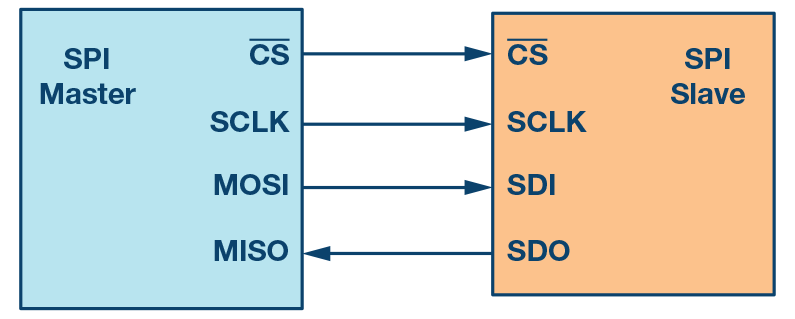
\includegraphics[width=.8\textwidth]{SPI-single.png}
  \end{center}
\end{frame}

\begin{frame} {SPI}
  Wichtige SPI-pins:
  \begin{itemize}
    \item CS - chip-select
    \item SCLK - Serial Clock
    \item MOSI - Master Out Slave In
    \item MISO - Master In Slave Out
  \end{itemize}
\end{frame}

\begin{frame} {SPI}
  \begin{itemize}
    \item Master gibt takt vor
    \item Slave nutzt Takt um Dinge zu tun
    \item Pro tick wird ein bit übermittelt
    \item Dies passiert im tausch!
  \end{itemize}
\end{frame}

\begin{frame} {SPI}
  \begin{center}
    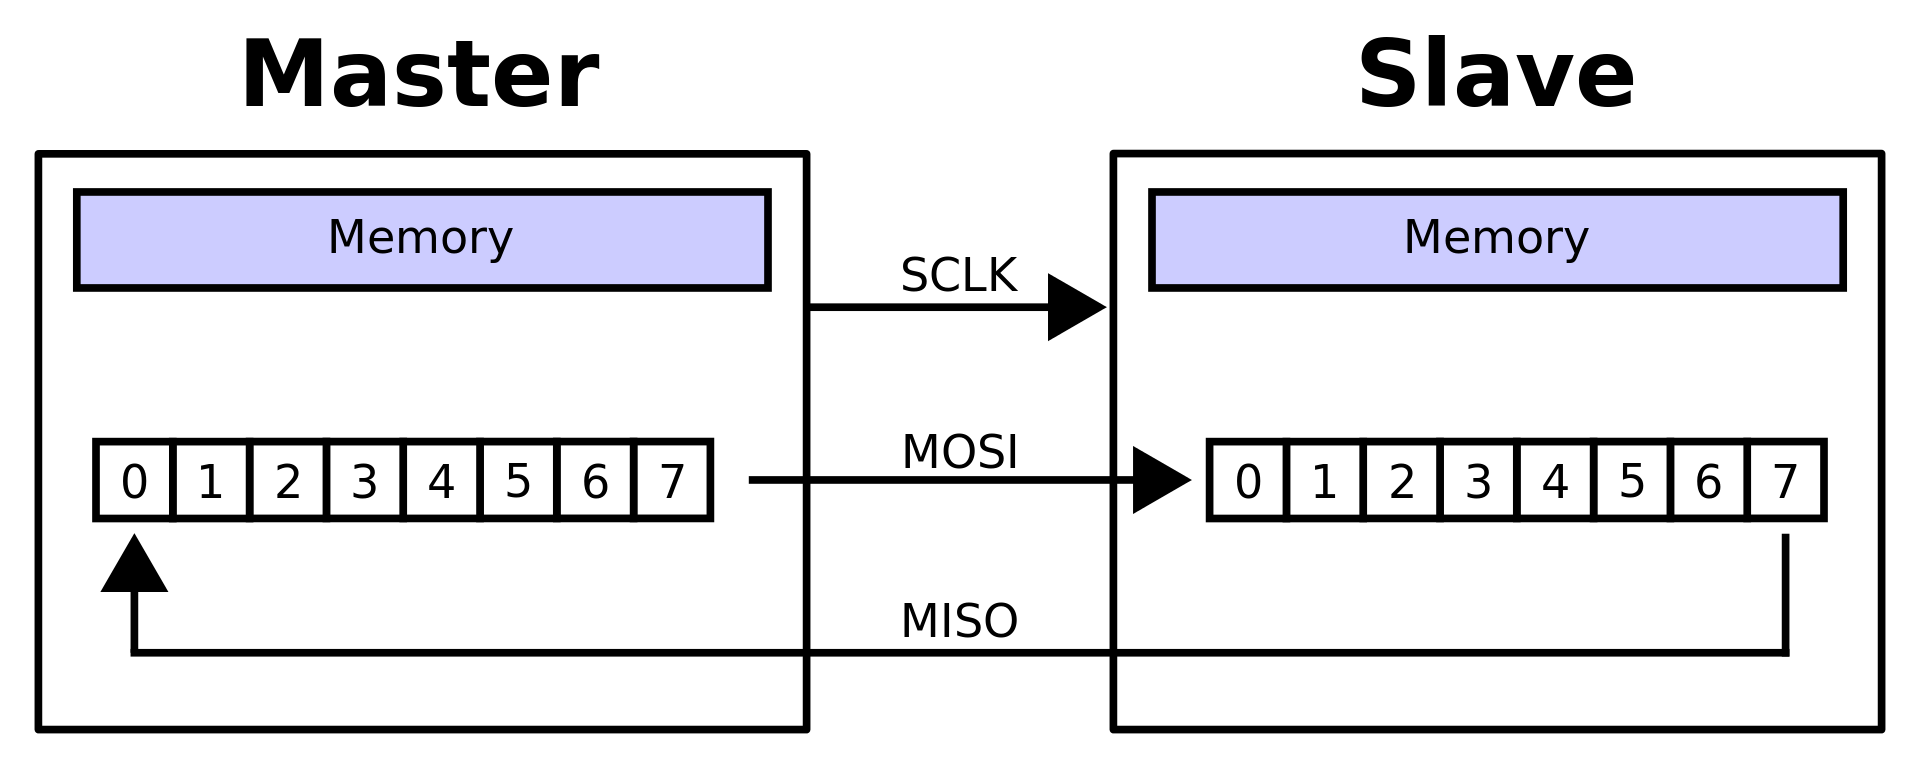
\includegraphics[width=\textwidth]{SPI-transfer}
  \end{center}
\end{frame}

\begin{frame} {SPI}
  \begin{itemize}
    \item SPI lässt auch mehrere Slaves zu
    \item CS - Chip Select pin wählt einen Slave zur Zeit
    \begin{itemize}
      \item[$\rightarrow$] Wichtig für die Aufgabe.
    \end{itemize}
  \end{itemize}
\end{frame}

\begin{frame} {SPI}
  \begin{center}
    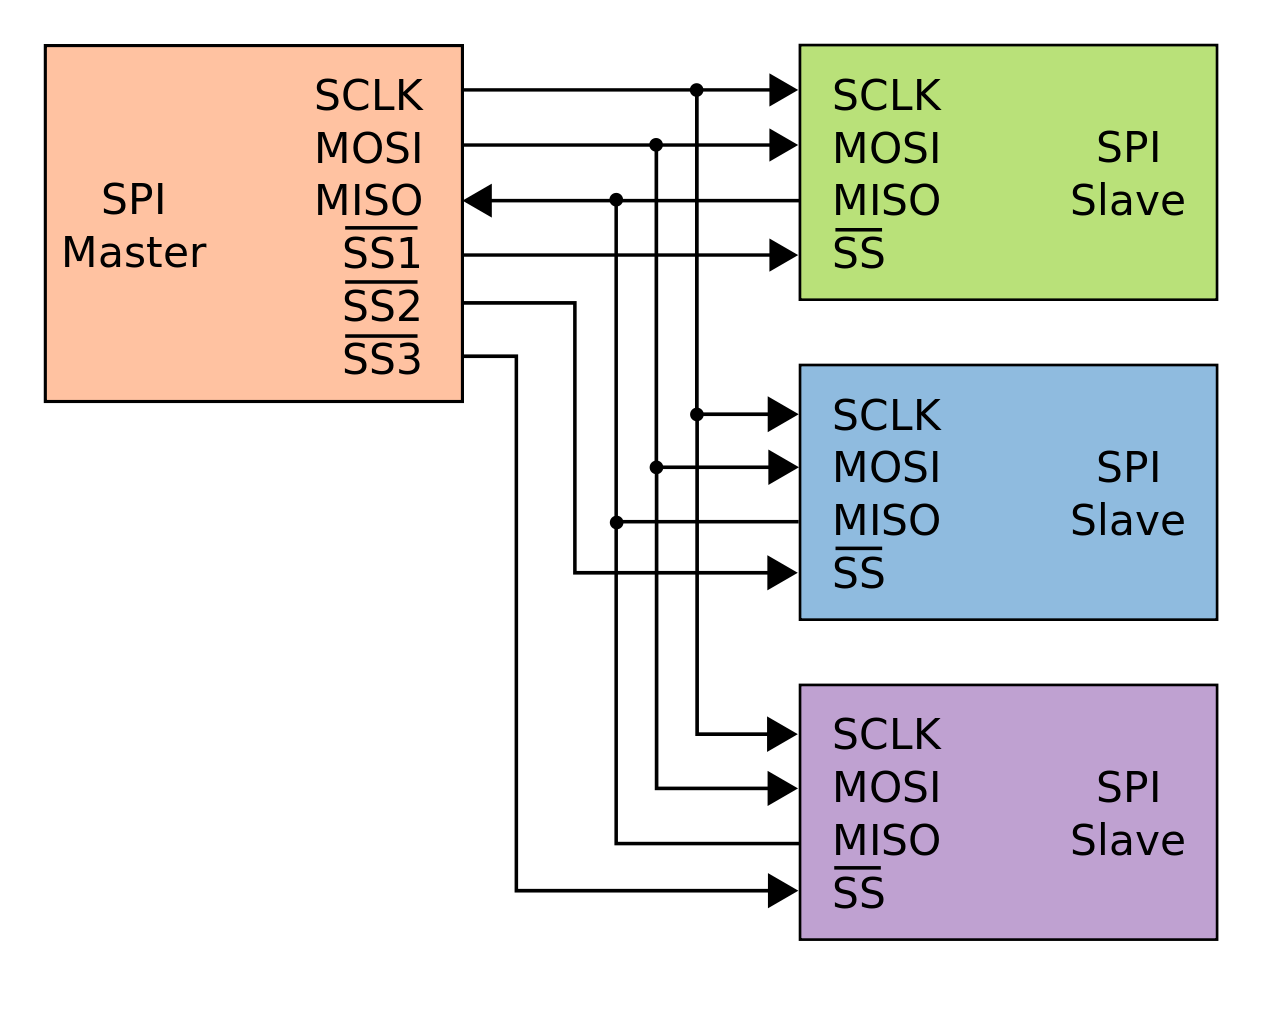
\includegraphics[height=.8\textheight]{SPI-parallel}    
  \end{center}
\end{frame}

\begin{frame} {SPI}
  \begin{center}
    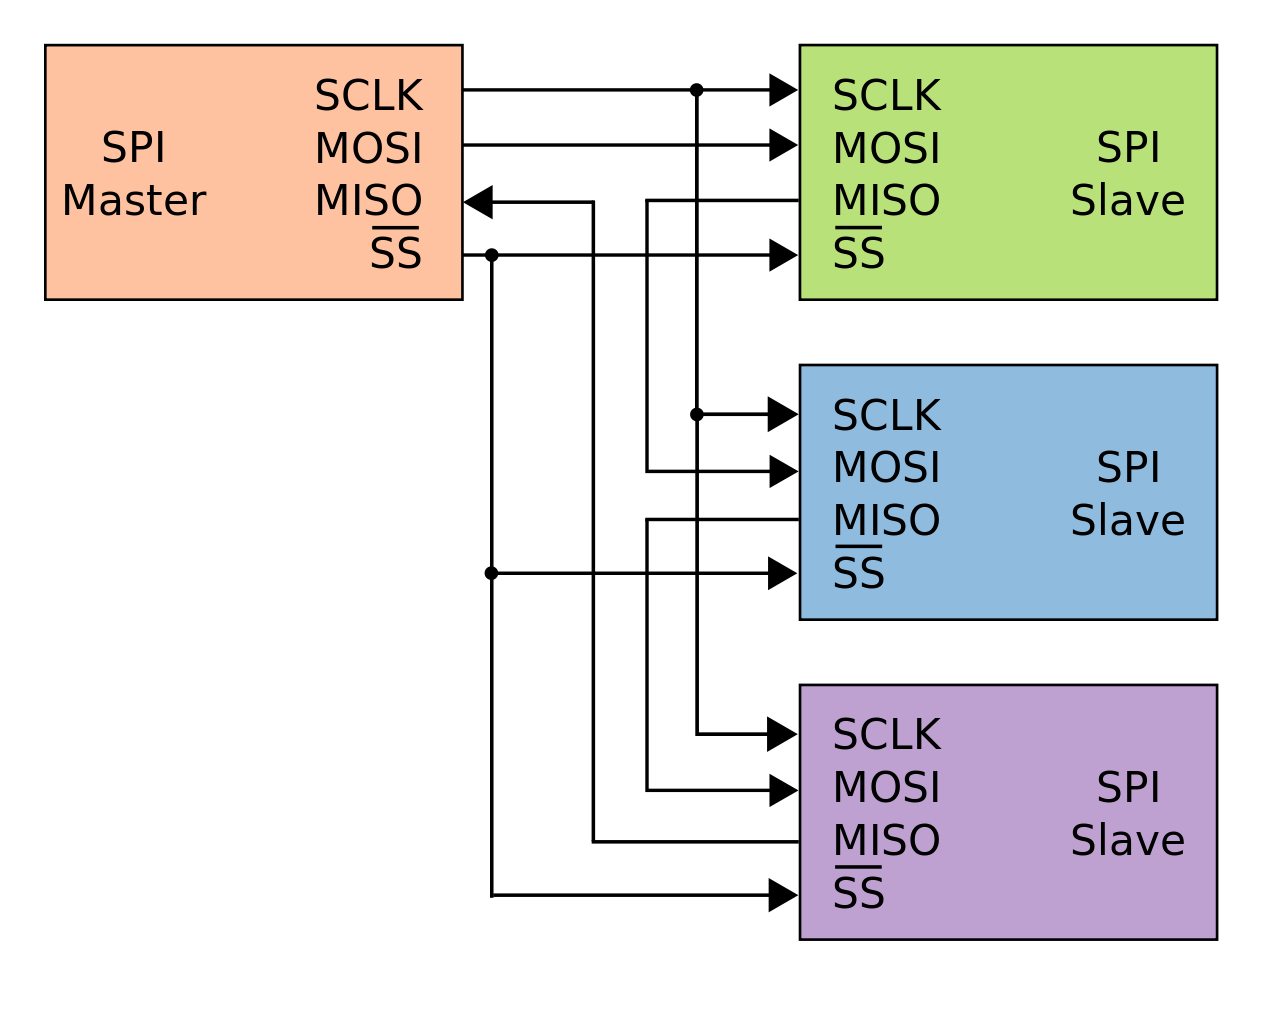
\includegraphics[height=.8\textheight]{SPI-daisychain}
  \end{center}
\end{frame}

\begin{frame} [fragile] {STM32-SPI}
  \begin{itemize}
    \item Praktischerweise alles geschenkt
    \item SPI ist in Hardware vorhanden
    \item lesen/schreiben:
    \begin{enumerate}
      \item byte in Dataregister schreiben
      \item warten auf Übertragungsende
      \item Daten zurückgeben
    \end{enumerate}
    \begin{lstlisting}
uint8_t spi_write_byte(uint8_t data) {
  SPI3->DR = data;
  while(!(SPI3->SR & SPI_SR_RXNE)); 
  return SPI3->DR;
}
      \end{lstlisting}
  \end{itemize}
\end{frame}

\sectionframe{\href{https://users.informatik.haw-hamburg.de/~schafers/LOCAL/S17S_CE/CODE/DemoSPI/main.c}{Beispielcode}}  

\section{Flash-Memory}
\sectionframe{\href{{https://users.informatik.haw-hamburg.de/~schafers/LOCAL/S19S_CE/DOCU/AT25DF641 Atmel 64MB SPI Serial Flash Memory Datasheet.pdf}}{Flash-Memory-Datasheet}}

\sectionframe{In der \href{https://owncloud.informatik.haw-hamburg.de}{\color{red}{owncloud}} gibts was einfacheres}

\end{document}